\documentclass[11pt,letterpaper]{article}

\usepackage[margin=0.9in]{geometry}
\usepackage{amsmath,amssymb,amsthm}
\usepackage{graphicx}
\usepackage{booktabs}
\usepackage{longtable}
\usepackage{array}
\usepackage{enumitem}
\usepackage[colorlinks=true,linkcolor=blue,citecolor=blue,urlcolor=blue]{hyperref}

\newtheorem{proposition}{Proposition}
\newtheorem{lemma}[proposition]{Lemma}
\DeclareMathOperator{\wrap}{wrap}
\DeclareMathOperator{\rnd}{round}
\DeclareMathOperator{\Var}{Var}
\DeclareMathOperator{\corr}{corr}
\DeclareMathOperator{\erfc}{erfc}
\newcommand{\PL}{P_{\mathrm{L}}}
\newcommand{\xpre}{x^{\mathrm{pre}}}

\setlist{itemsep=2pt,topsep=3pt}

\title{Validation of the GKP simulator (\texttt{simulator/sim.py})}
\date{November 2026}

\begin{document}
\maketitle

This note defines the model that \texttt{sim.py} simulates and derives every
reference value used to test it. For each one it says where the value comes
from (a closed form or a published result), and then compares the simulator
against it. Everything can be reproduced from the repo root with
\begin{center}
\texttt{python -m experiments.validate\_sim}
\end{center}

\begin{figure}[h]
  \centering
  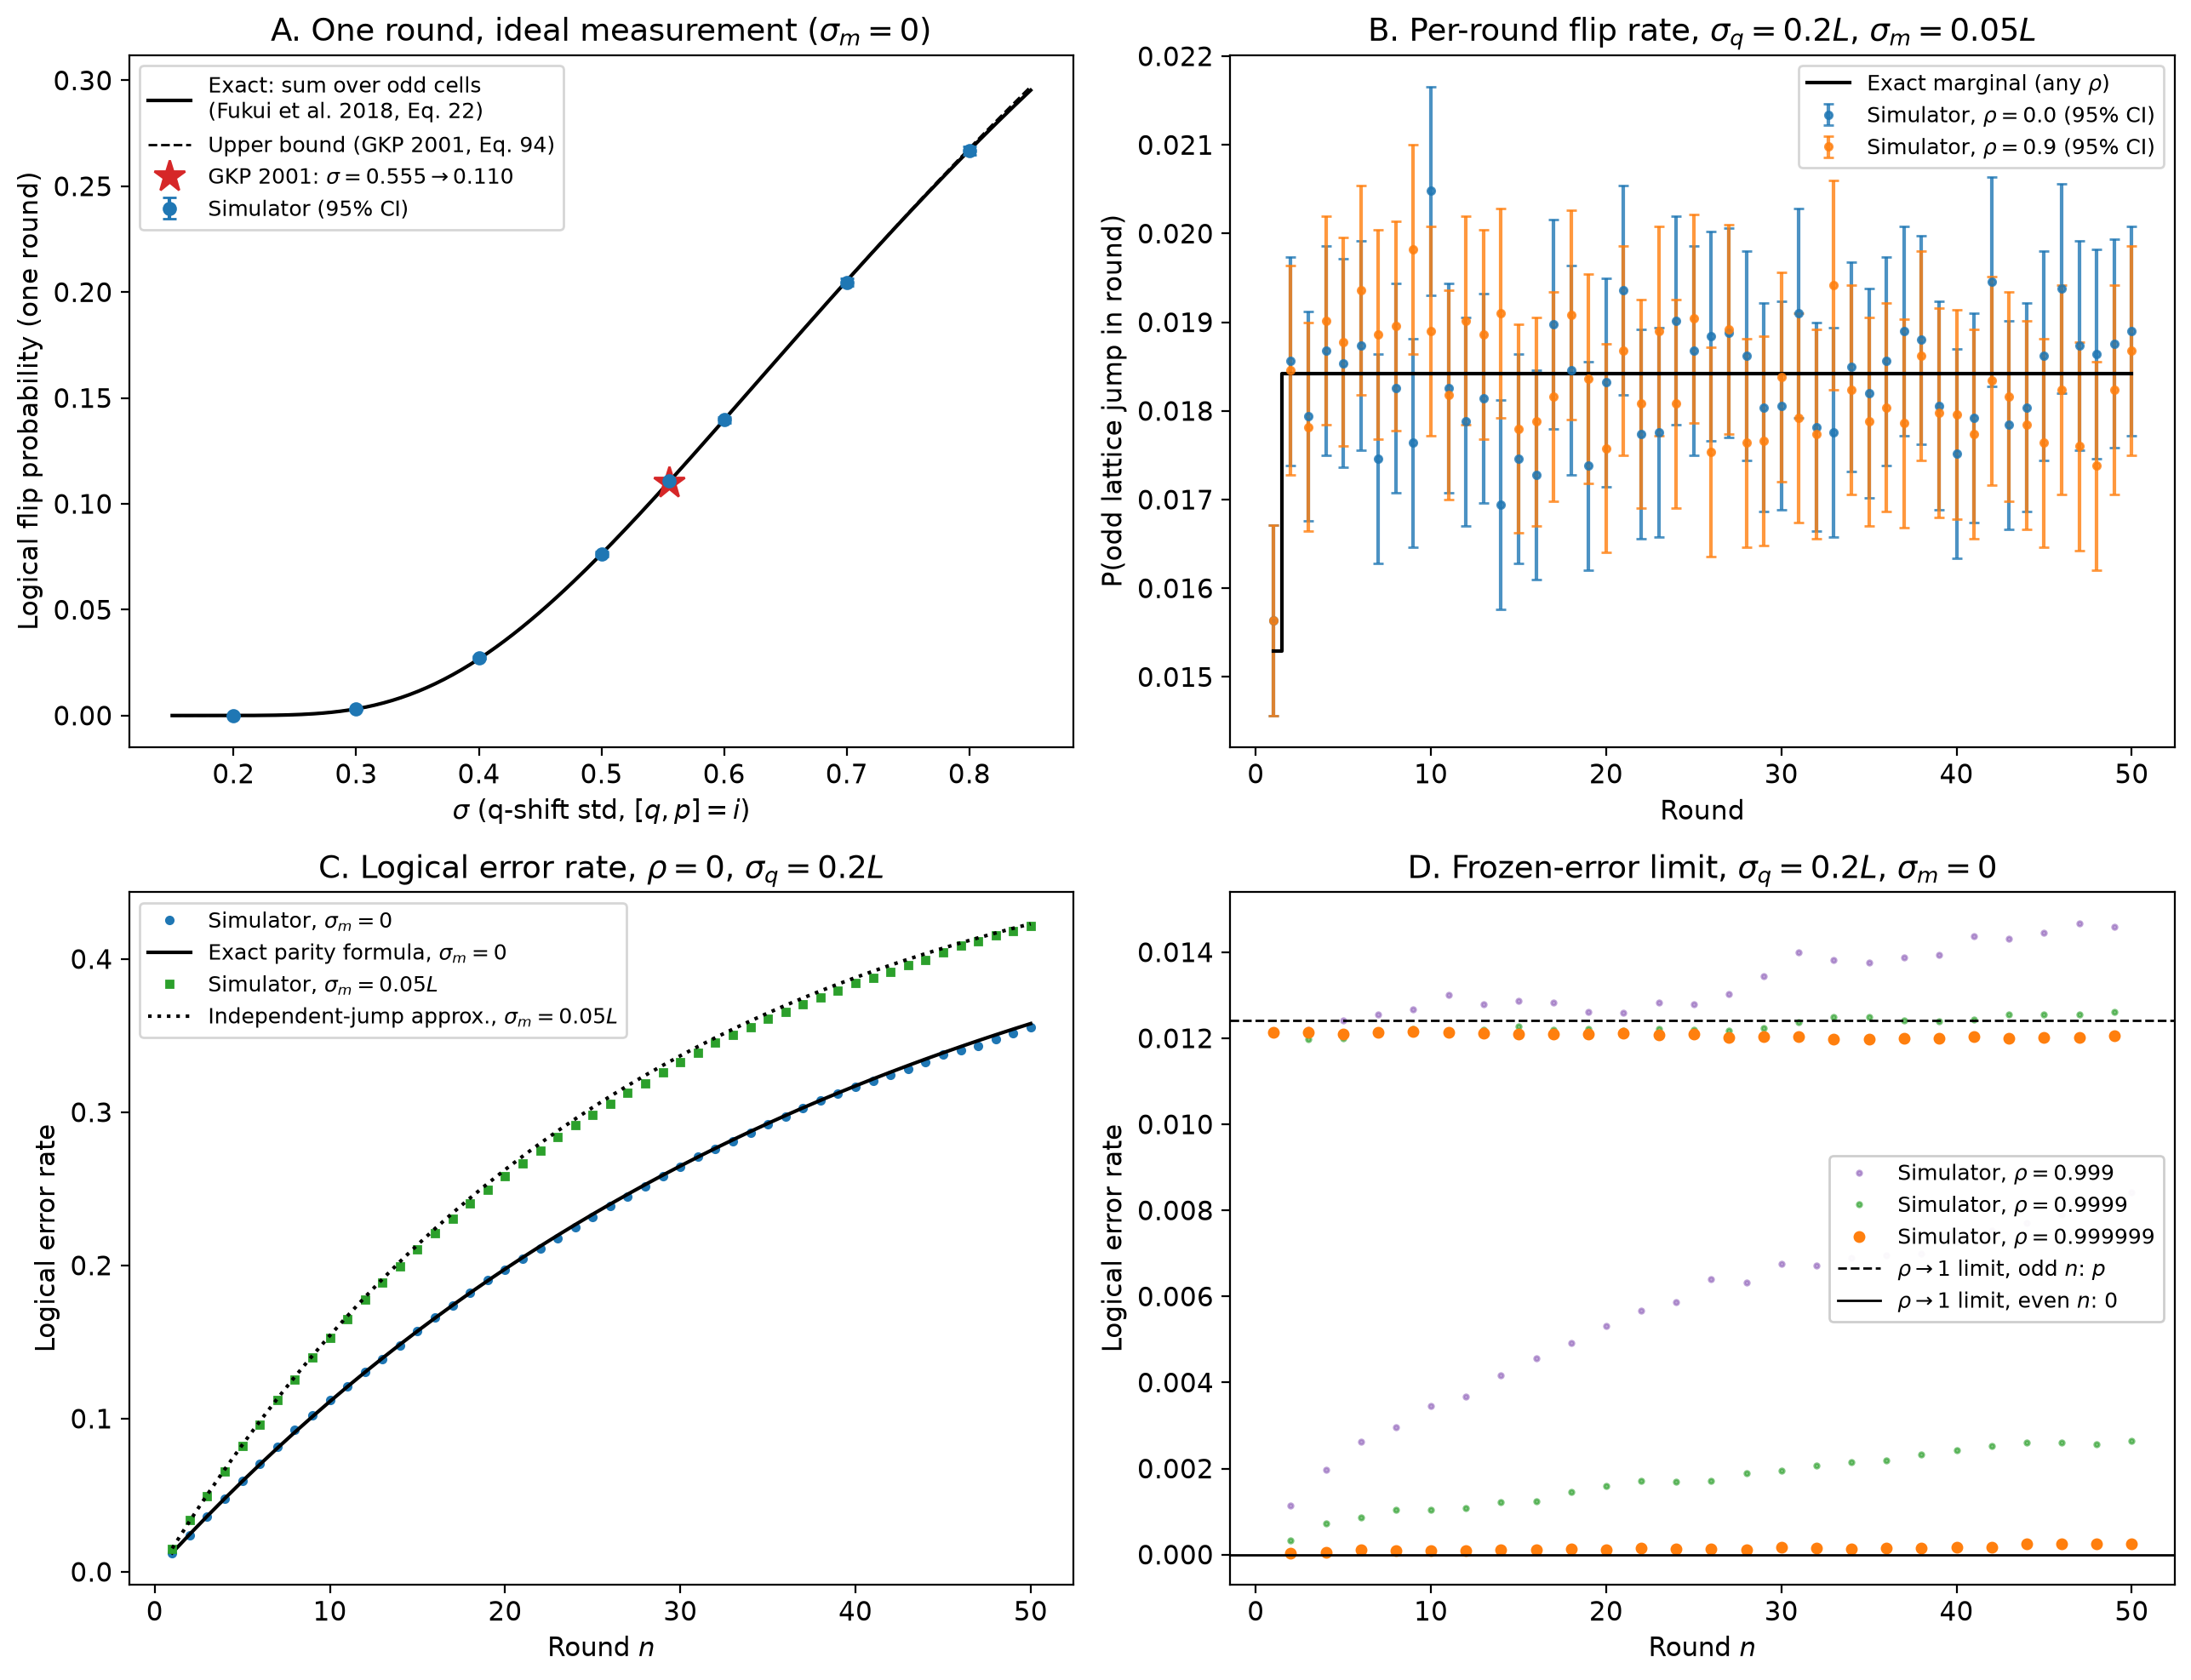
\includegraphics[width=0.92\textwidth]{figures/sim_validation.png}
  \caption{Simulator (markers) against closed-form references (lines).
  A: single round, ideal measurement. B: per-round flip rate.
  C: logical error rate for $\rho=0$. D: frozen-error limit $\rho\to1$.}
\end{figure}

%-------------------------------------------------------------------
\section{Model}

\paragraph{Conventions.}
We use dimensionless quadratures with $[\hat q,\hat p]=i$ ($\hbar=1$) and the
square GKP code, which has stabilizer $S_q=e^{2i\sqrt\pi\,\hat q}$ and lattice
spacing
\[
  L=\sqrt\pi .
\]
Logical $|\bar 0\rangle$ has position peaks at $q=2nL$, and $|\bar 1\rangle$
has them at $q=(2n+1)L$. A shift by $2L$ is therefore a stabilizer (no
effect), a shift by $L$ is the logical $\bar X$, and a shift with $|r|<L/2$ is
correctable. This is the convention of Gottesman--Kitaev--Preskill~[1].
Throughout, $\sigma$ means the standard deviation of the physical $q$-shift in
this convention (see Section~\ref{sec:sources} for the factor $\sqrt2$ in
Grimsmo--Puri~[3]).

\paragraph{Noise} (\texttt{simulator/noise.py}, \texttt{NoiseModel}).
For each trial and round $t=1,\dots,T$:
\begin{align*}
  \varepsilon_1 &\sim \mathcal N(0,\sigma_q^2), &
  \varepsilon_t &= \rho\,\varepsilon_{t-1}+\eta_t, \quad
  \eta_t \sim \mathcal N\!\bigl(0,\sigma_q^2(1-\rho^2)\bigr), \\
  \nu_t &\sim \mathcal N(0,\sigma_m^2) \text{ i.i.d.}
\end{align*}
Hence $\Var\varepsilon_t=\sigma_q^2$ for every $t$ and every $\rho\in(-1,1)$;
the AR(1) process is stationary.

\paragraph{Error-correction round} (\texttt{Simulator.run}).
Starting from residual $x_0=0$:
\begin{align*}
  \xpre_t &= x_{t-1}+\varepsilon_t && \text{(displacement error)}\\
  s_t &= \wrap(\xpre_t+\nu_t) && \text{(noisy syndrome)}\\
  c_t &= \mathcal D(s_1,\dots,s_t) && \text{(decoder)}\\
  x_t &= \xpre_t-c_t && \text{(correction)}
\end{align*}
with $\wrap(y)=y-L\,\rnd(y/L)\in[-L/2,L/2)$.

\paragraph{Logical error after round $t$.}
Write $x_t=k_tL+r_t$, where $k_t=\rnd(x_t/L)$ and $|r_t|<L/2$. A single ideal
final correction removes $r_t$, while $k_tL$ applies $\bar X^{k_t}$. Hence
\[
  \text{logical error after round } t \iff k_t \text{ is odd}.
\]
The logical error rate is $\PL(t)=\Pr[k_t\text{ odd}]$
(\texttt{SimResult.logical\_error\_rate}), and the lattice jump in round $t$ is
$\Delta k_t=k_t-k_{t-1}$ (\texttt{SimResult.lattice\_jumps}).
The \emph{nearest-lattice decoder} sets $c_t=s_t$.

%-------------------------------------------------------------------
\section{Closed-form results for the nearest-lattice decoder}

Let $\Phi$ be the standard normal CDF. For $Z\sim\mathcal N(0,\sigma^2)$
define
\begin{equation}
  \boxed{\;
  p(\sigma)=\Pr\bigl[\rnd(Z/L)\text{ odd}\bigr]
  =\sum_{j\text{ odd}}\left[
     \Phi\!\left(\frac{(j+\tfrac12)L}{\sigma}\right)
    -\Phi\!\left(\frac{(j-\tfrac12)L}{\sigma}\right)\right]
  \;}
  \tag{P}\label{eq:P}
\end{equation}
(\texttt{sim.odd\_jump\_probability}). The cells $|j|\ge3$ contribute
exponentially little, so
\[
  p(\sigma)\approx 2\bigl[1-\Phi(L/2\sigma)\bigr]
  =\erfc\!\left(\frac{L}{2\sqrt2\,\sigma}\right),
\]
and this tail is also an upper bound on $p(\sigma)$.

\begin{proposition}[Single round, ideal measurement]\label{prop:single}
If $\sigma_m=0$, a single round ends in a logical error with probability
$p(\sigma_q)$.
\end{proposition}
\begin{proof}
$\xpre_1=\varepsilon_1$ and $c_1=\wrap(\varepsilon_1)$, so
$x_1=L\,\rnd(\varepsilon_1/L)$ and $k_1=\rnd(\varepsilon_1/L)$.
\end{proof}

\noindent\emph{Literature.} \eqref{eq:P} is the incorrect-decision
probability of Fukui et al.~[2], Eq.~(22), at cutoff $v_{\mathrm{up}}=0$.
GKP~[1], Eq.~(94), gives the bound
$p_e<\erfc\bigl(\sqrt\pi/(2\sqrt2\sigma)\bigr)$ and evaluates it as $0.110$ at
$\sigma\approx0.555$. Both papers use the same $\sigma$ convention and the
same $\sqrt\pi$ lattice as this note.

\begin{lemma}[Residual after a nearest-lattice correction]\label{lem:residual}
For every noise realisation,
\[
  x_t = L\,\rnd\!\bigl((\xpre_t+\nu_t)/L\bigr)-\nu_t .
\]
\end{lemma}
\begin{proof}
$x_t=\xpre_t-\wrap(\xpre_t+\nu_t)
=\xpre_t-(\xpre_t+\nu_t)+L\,\rnd\bigl((\xpre_t+\nu_t)/L\bigr)$.
\end{proof}

After every round, then, the oscillator sits on a lattice point shifted by
minus that round's measurement error. When $|\nu_t|<L/2$ (almost surely
here, since $\sigma_m=0.05L$), we have $k_t=\rnd\bigl((\xpre_t+\nu_t)/L\bigr)$.

\noindent\emph{Status.} The lemma follows from the model by direct algebra. We
did not find it stated in this form in~[1--3]. Grimsmo--Puri~[3] (Fig.~10,
Sec.~III.2) describe the related fact that a measurement error leaves a small
residual displacement after correction.

\begin{proposition}[Per-round flip probability, any $\rho$]\label{prop:perround}
\[
  \Delta k_t=\rnd(z_t/L),\qquad
  z_t=\varepsilon_t+\nu_t-\nu_{t-1}\quad(\nu_0\equiv0),
\]
and therefore
\[
  \Pr[\Delta k_t\text{ odd}]=
  \begin{cases}
    p\bigl(\sqrt{\sigma_q^2+\sigma_m^2}\bigr), & t=1,\\[3pt]
    p\bigl(\sqrt{\sigma_q^2+2\sigma_m^2}\bigr), & t\ge2.
  \end{cases}
\]
\end{proposition}
\begin{proof}
Substitute $x_{t-1}=k_{t-1}L-\nu_{t-1}$ (Lemma~\ref{lem:residual}) into
$\xpre_t$; the $k_{t-1}L$ term is a lattice multiple and drops out of the
rounding. The variable $z_t$ is a sum of independent Gaussians:
$\varepsilon_t$ has variance $\sigma_q^2$ for every $\rho$, and $\nu_t$ and
$\nu_{t-1}$ are independent of it.
\end{proof}

This describes the \emph{marginal of a single round} only. When $\rho\ne0$,
the jumps $\Delta k_t$ in different rounds are correlated.

\begin{proposition}[Logical error rate for independent jumps]\label{prop:parity}
If the parities of $\Delta k_1,\dots,\Delta k_n$ are independent, with odd
probabilities $p_1,\dots,p_n$, then
\[
  \PL(n)=\tfrac12\Bigl[1-\prod_{t=1}^{n}(1-2p_t)\Bigr].
\]
\end{proposition}
\begin{proof}
$k_n=\sum_t\Delta k_t$, so
$\mathbb E[(-1)^{k_n}]=\prod_t\mathbb E[(-1)^{\Delta k_t}]=\prod_t(1-2p_t)$.
\end{proof}

This is the standard parity (``piling-up'') identity for independent bits. It
applies to our model as follows.
\begin{itemize}
  \item \textbf{Exact} when $\rho=0$ and $\sigma_m=0$: the $z_t=\varepsilon_t$ are
    i.i.d., so $\PL(n)=\frac12\bigl[1-(1-2p(\sigma_q))^n\bigr]$.
  \item \textbf{Approximate} when $\rho=0$ and $\sigma_m>0$: $z_t$ and $z_{t+1}$
    share $\nu_t$ with opposite signs, so
    $\corr(z_t,z_{t+1})=-\sigma_m^2/(\sigma_q^2+2\sigma_m^2)\approx-0.056$ for
    the default parameters. We use $p_1=p\bigl(\sqrt{\sigma_q^2+\sigma_m^2}\bigr)$
    and $p_{t\ge2}=p\bigl(\sqrt{\sigma_q^2+2\sigma_m^2}\bigr)$.
  \item \textbf{Not valid} when $\rho\ne0$. We claim no closed form there.
\end{itemize}

\begin{proposition}[Frozen-error limit $\rho\to1$, $\sigma_m=0$]\label{prop:frozen}
If $\varepsilon_t\equiv\varepsilon$ for all $t$, every round jumps by
$\rnd(\varepsilon/L)$. Then $k_n=n\,\rnd(\varepsilon/L)$, and
\[
  \PL(n)=
  \begin{cases}
    p(\sigma_q), & n\text{ odd},\\
    0, & n\text{ even}.
  \end{cases}
\]
\end{proposition}
The simulator requires $|\rho|<1$, so we check this as a limit, letting
$\rho$ approach~1.

%-------------------------------------------------------------------
\section{Results}

Unless noted otherwise, the parameters are $\sigma_q=0.2L$ and
$\sigma_m=0.05L$, with 200\,000 trials for check~A, 50\,000 trials for
checks~B--D, and seed 2026. The score is
$z=(\hat p-p)/\sqrt{p(1-p)/N}$, computed with the reference value $p$.

{\footnotesize
\setlength{\tabcolsep}{4pt}
\begin{longtable}{@{}p{3.5cm}p{4.3cm}rrrl@{}}
\toprule
Check & Case & Simulated & Reference & $z$ & Type \\
\midrule
\endhead
A: single round & $\sigma=0.200$ & 0.00001 & 0.00001 & $-0.64$ & exact \\
(Prop.~\ref{prop:single}) & $\sigma=0.300$ & 0.00298 & 0.00314 & $-1.21$ & exact \\
 & $\sigma=0.400$ & 0.02739 & 0.02672 & $+1.87$ & exact \\
 & $\sigma=0.500$ & 0.07616 & 0.07632 & $-0.26$ & exact \\
 & $\boldsymbol{\sigma=0.555}$ & \textbf{0.11076} & \textbf{0.11031} & $+0.64$ & exact + lit. \\
 & & & (GKP: 0.110) & & \\
 & $\sigma=0.600$ & 0.13967 & 0.13965 & $+0.01$ & exact \\
 & $\sigma=0.700$ & 0.20458 & 0.20535 & $-0.86$ & exact \\
 & $\sigma=0.800$ & 0.26687 & 0.26707 & $-0.20$ & exact \\
\midrule
B: per-round flip & $\rho=0$, round 1 & 0.01564 & 0.01529 & $+0.63$ & exact \\
(Prop.~\ref{prop:perround}) & $\rho=0$, mean of rounds 2--50 & 0.01837 & 0.01842 & $-0.66$ & exact \\
 & $\rho=0.9$, round 1 & 0.01564 & 0.01529 & $+0.63$ & exact \\
 & $\rho=0.9$, mean of rounds 2--50 & 0.01834 & 0.01842 & $-1.01$ & exact \\
\midrule
C1: $\PL$, $\rho=0$, $\sigma_m=0$ & worst of 50 rounds (47) & 0.34344 & 0.34669 & $-1.53$ & exact \\
(Prop.~\ref{prop:parity}) & round 50 & 0.35562 & 0.35783 & $-1.03$ & exact \\
\midrule
C2: $\PL$, $\rho=0$, $\sigma_m=0.05L$ & round 50 & 0.42174 & 0.42298 & $-0.56$ & approx. \\
\midrule
D: $\rho\to1$, $\sigma_m=0$ & $\rho=0.999$, odd / even $n$ & 0.01330 / 0.00561 & 0.01242 / 0 & & limit \\
(Prop.~\ref{prop:frozen}) & $\rho=0.9999$, odd / even $n$ & 0.01230 / 0.00174 & 0.01242 / 0 & & limit \\
 & $\rho=0.99999$, odd / even $n$ & 0.01207 / 0.00052 & 0.01242 / 0 & & limit \\
 & $\rho=0.999999$, odd / even $n$ & 0.01207 / 0.00015 & 0.01242 / 0 & & limit \\
\bottomrule
\end{longtable}
}

\paragraph{A (panel A).} All eight points lie within $2$ standard errors of the
reference. At $\sigma=0.555$ the exact sum~\eqref{eq:P} and the GKP bound
agree to four decimals ($0.1103$). The bound also counts the even cells
$|j|\ge2$, but they add only $1.7\times10^{-6}$. This reproduces GKP's quoted
value of $0.110$.

\paragraph{B (panel B).} Round~1 gives the same number for both values of
$\rho$. This is by design: the two runs share a seed, and $\varepsilon_1$ does
not depend on $\rho$. The pooled $z$ for rounds 2--50 assumes the rounds are
independent, which they are not, so treat it as indicative only. Taken round
by round, the most extreme of the 49 rounds has $|z|=3.42$ for $\rho=0$
(Bonferroni $p=0.03$) and $|z|=2.32$ for $\rho=0.9$ ($p=0.99$). We reran
$\rho=0$ with three more seeds and got a maximum $|z|$ of $2.60$, $3.30$ and
$2.96$, while the mean over rounds 2--50 stayed between $0.01835$ and
$0.01840$ (exact value $0.01842$). We read the large single-round values as
the result of picking the most extreme of 49 rounds, not as a bias.

\paragraph{C (panel C).} With $\sigma_m=0$ the simulator follows the exact
curve for all 50 rounds. With $\sigma_m>0$ it lies slightly \emph{below} the
independent-jump approximation, which is the predicted direction:
$z_t$ and $z_{t+1}$ are negatively correlated, so jumps tend to come in
$+1,-1$ pairs that cancel in parity.

\paragraph{D (panel D).} The odd-round rate approaches
$p(\sigma_q)=0.0124$ and the even-round rate approaches $0$. The leftover
even-round rate falls by about $\sqrt{10}$ for every factor of 10 reduction
in $1-\rho$. That fits a picture in which $\varepsilon_t$ drifts by about
$\sigma_q\sqrt{1-\rho^2}$ per round.

\paragraph{Conclusion.} The simulator reproduces every closed-form and
literature value in this note within statistical error. Where only an
approximation or a limit is available, it deviates in the predicted direction
and converges as predicted.

%-------------------------------------------------------------------
\section{What is \emph{not} validated here}

\begin{itemize}
  \item For $0<\rho<1$ there is \textbf{no closed form} here for the logical
    error rate over many rounds. Those curves, for example the drop from
    $0.425$ at $\rho=0$ to $0.247$ at $\rho=0.9$ after 50 rounds, come from
    the simulator alone. They are consistent with
    Propositions~\ref{prop:perround}--\ref{prop:frozen}, which cover the
    per-round marginal and the two ends $\rho=0$ and $\rho\to1$.
  \item Decoders other than nearest-lattice and no correction.
  \item Anything beyond the classical shift model: finite-energy ($\Delta$)
    effects, $p$-quadrature noise, ancilla noise in the extraction circuit,
    and loss. \texttt{quantum/encoding.py} is the starting point for checking
    the shift model against QuTiP.
\end{itemize}

%-------------------------------------------------------------------
\section{Sources and conventions}\label{sec:sources}

{\small
\renewcommand{\arraystretch}{1.25}
\begin{tabular}{@{}>{\raggedright\arraybackslash}p{2.6cm}>{\raggedright\arraybackslash}p{3.6cm}>{\raggedright\arraybackslash}p{4.0cm}>{\raggedright\arraybackslash}p{5.0cm}@{}}
\toprule
Ref. & Used for & Location & $\sigma$ convention \\
\midrule
{[1]} GKP 2001 & Bound; value $0.110$ at $\sigma=0.555$ & Sec.~VIII, Eqs.~(94)--(95)
  & std of physical $q$-shift, $[q,p]=i$, $\hbar=1$ (same as here) \\
{[2]} Fukui et al.\ 2018 & Exact odd-cell sum~\eqref{eq:P} & Sec.~III.2, Eq.~(22), $v_{\mathrm{up}}=0$
  & std of $q$-deviation, $\sqrt\pi$ lattice (inferred; not stated) \\
{[3]} Grimsmo \& Puri 2021 & Code conventions; residual-shift picture & Eqs.~(4), (5a), (26); Sec.~III.2; Fig.~10
  & $\sigma$ per component of $\zeta$ in $D(\zeta)$; \textbf{physical $q$-std is $\sqrt2\,\sigma$} \\
\bottomrule
\end{tabular}
}

\medskip
We derived Lemma~\ref{lem:residual} and
Propositions~\ref{prop:perround}--\ref{prop:frozen}, with their proofs, from
the model in Section~1. We did not find them stated in this form in~[1--3].
The equation and section numbers were read from the arXiv HTML versions
listed below (GKP v3; Fukui v3, of which only the first half was read
verbatim; Grimsmo--Puri v1). Check them against the journal versions before
citing.

\begin{enumerate}[label={[\arabic*]}]
  \item D.~Gottesman, A.~Kitaev, J.~Preskill, ``Encoding a qubit in an
    oscillator,'' \emph{Phys.\ Rev.\ A} \textbf{64}, 012310 (2001).
    \url{https://arxiv.org/abs/quant-ph/0008040}
  \item K.~Fukui, A.~Tomita, A.~Okamoto, K.~Fujii, ``High-threshold
    fault-tolerant quantum computation with analog quantum error correction,''
    \emph{Phys.\ Rev.\ X} \textbf{8}, 021054 (2018).
    \url{https://arxiv.org/abs/1712.00294}
  \item A.~L.~Grimsmo, S.~Puri, ``Quantum error correction with the
    Gottesman--Kitaev--Preskill code,'' \emph{PRX Quantum} \textbf{2}, 020101
    (2021). \url{https://arxiv.org/abs/2106.12989}
\end{enumerate}

\end{document}
